\chapter{Thermal Expansion}
\label{ch:thermalExpansion}

\section{Necessity of Modeling}
  The Fast Reactor (FR) as modeled is entirely composed of
  metals and, as such, experiences significant thermal expansion. While other 
  designs may employ non-metallic fuel material (e.g. oxides or carbides), these 
  are not considered. Reactor designs with metal fuel include 
  Experimental Breeder Reactor II (EBR-II) as designed and built by Argonne 
  National Laboratory (ANL) and PRISM as designed by GE-Hitachi Nuclear Energy 
  (GEH).

  In metal fueled reactors such as EBR-II and PRISM, thermal expansion 
  represents a significant feedback effect and requires modeling. PRISM 
  estimates a thermal expansion feedback such that a 1\% change in radial 
  dimension results in $-0.5 \units{$\Delta k$}$ indicating a significant effect 
  \cite{GEFR793}. Additionally, thermal expansion has been proven to serve as an 
  inherent safety feature of SFRs. In the remarkable EBR-II demonstrations in 
  April 1986, two major accident events were performed on the reactor while 
  operating at full power. Operators forced the reactor to undergo Unprotected 
  Loss-Of-Flow (ULOF) and Unprotected Loss-Of-Heat-Sink (ULOHS) events. EBR-II 
  was safely shutdown due to nothing other than inherent thermal feedback 
  effects. These experiments demonstrated conclusively the passive safety of SFR
  designs due in part to the thermal expansion of materials 
  \cite{PlentifulEnergy}.

\section{Model Details}
  \label{sec:model_details}
  Highly detailed thermal expansion modeling can be performed using the Finite
  Element Method (FEM) to calculate local stresses and strains on all reactor
  structural components such as fuel pins, wire wraps, and assembly boxes. 
  However, the model developed here for the simulation of
  fast reactors does not estimate temperature and heat generation at all 
  positions due to the smearing of hexagonal assemblies. Therefore, a simplified 
  thermal expansion model is developed to simulate the effect of thermal 
  expansion on reactivity.

  In the model, linear dimensions are expanded based on material properties.
  All sodium in the reactor is assumed to be liquid so effects of thermal
  expansion within the sodium are assumed to be described by the change in
  density as a function of temperature as described by state equations in
  \cite{sodiumProp}. Additionally, the mass of sodium within the reactor is not
  conserved. In a Sodium-cooled Fast Reactor (SFR), sodium in the coolant is 
  allowed to flow into and out of an expansion vessel external to the reactor.
  The sodium in the bond region flows upward from the fuel region into a gas 
  plenum at the top of the fuel rod as the fuel expands. However, this is not 
  modeled as the sodium level in the bond is not tracked. Instead, the mass of 
  sodium in the bond region is allowed to vary during the simulation.

  \subsection{Material Properties}
    \label{sec:model_details__material_properties}
    All structural materials in the reactor are thermally expanded as HT9 
    stainless steel.
    Fuel material is thermally expanded as metallic uranium with 10\% Zr by 
    weight included (i.e. U10Zr). Thermal expansion properties for HT9 are given 
    in \cite{ht9Prop} and for U10Zr are given in \cite{thexpU10Zr}. The 
    equations for the Linear Expansion Factor (LEF) as functions of temperature 
    and used in this implementation are given
    \begin{equation}
      \label{eq:lef_ht9}
      \left( \frac{\Delta L}{L} \right)_{\text{HT9}} = 
        -2.191 \times 10^{-3} + 5.678 \times 10^{-6} \, T + 
        8.111 \times 10^{-9} \, T^2 - 2.576 \times 10^{-12} \, T^3 ,
    \end{equation}
    \begin{multline}
      \label{eq:lef_u10zr}
      \left( \frac{\Delta L}{L} \right)_{\text{U10Zr}} = \\
        \begin{cases}
          -7.3 \times 10^{-3} + 3.489 \times 10^{-5} \, T 
            - 5.154 \times 10^{-8} \, T^2 + 4.39 \times 10^{-11} \, T^3 & 
            T \le 923 \units{K} \\
          -0.25252 + 6.669 \times 10^{-4} \, T - 5.441 \times 10^{-7} \, T^2 
            + 1.518 \times 10^{-10} \, T^3 & \text{otherwise}
        \end{cases}
    \end{multline}
    for $T$ in \units{K}. Note that U10Zr undergoes a phase change at 
    $923 \units{K}$ that increases the LEF at this point. The LEF of HT9 and 
    U10Zr over the range of operating temperatures of fast reactors are plotted 
    in \fref{fig:lef_plot}. It is observed that the LEF of U10Zr is as much as 
    twice that of HT9. This implies fuel material will expand significantly more 
    than structural material which is expected behavior for metallic fuel.

    \begin{figure}
      \centering
      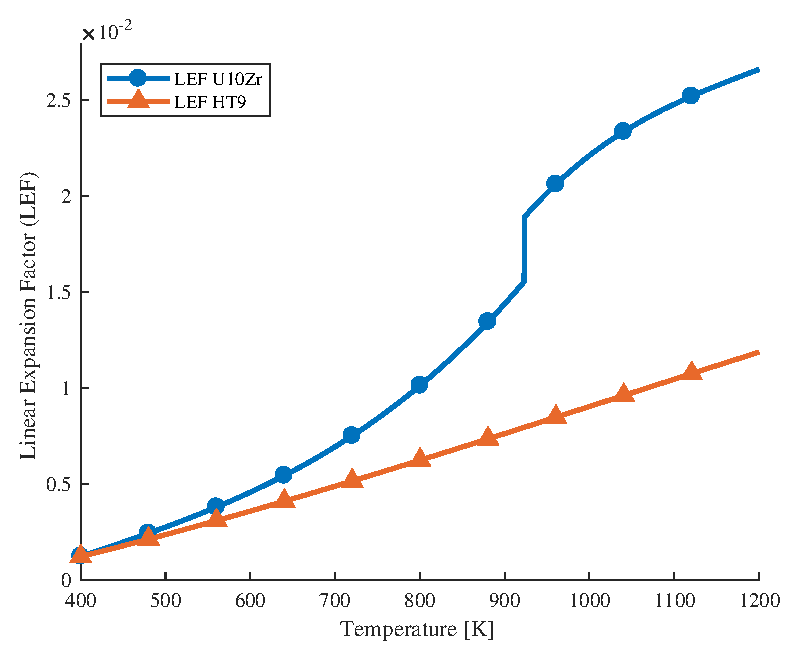
\includegraphics[width=0.7\textwidth]{lef_plot}
      \caption{Linear Expansion Factor for HT9 Steel and U10Zr Fuel.}
      \label{fig:lef_plot}
    \end{figure}
    
  \subsection{Assumptions and Formulae}
  \label{sec:model_details__assumptions_and_formulae}
    To simplify the modeling of thermal expansion, material dimensions are
    uniformly expanded in radial and axial directions. It is assumed that 
    material expansion in the radial direction (both $x$ and $y$ directions) 
    expands as HT9 because the dominating expansion in this direction is due to 
    the expansion of the hexagonal assemblies themselves and the grid plate at
    the base of the reactor. The exception to radial thermal expansion is that 
    the radius of the fuel, $R_F$, expands as U10Zr.  Within a hexagonal 
    assembly, the coolant flow area and the sodium bond area are allowed to 
    vary because of the assumption that the sodium is liquid.  It is assumed 
    that material expansion in the axial direction (the $z$ direction) expands 
    as U10Zr because the dominating expansion in this direction is the 
    elongation of the metallic fuel.
    
    All dimensions in the reactor are expanded assuming the user-input 
    dimensions are at room-temperature conditions. Dimensions are expanded
    according to two user-input temperatures, $\texpfuel$ and $\texpstruct$.
    $\texpfuel$ corresponds to the average temperature of reactor fuel and
    $\texpstruct$ corresponds to the average temperature of steel in the
    reactor. Typically, these values come from a previous coupled diffusion and
    thermal hydraulics simulation and must be known before the simulation 
    begins. It is expected thermal expansion effects will be significant. 
    However, thermal expansion factors are typically on the order $10^{-6}$ so 
    small, local changes in temperature are not expected to affect the 
    macroscopic simulation.

    Given the assumptions of this model, a radial LEF can be defined using 
    \eref{eq:lef_ht9} as
    \begin{equation}
      \label{eq:lef_r}
      F_r(\texpstruct) = \left(\frac{\Delta L}{L}\right)_{\text{HT9}}
    \end{equation}
    which is a function of $\texpstruct$. Note that given the assumption of 
    uniform radial thermal expansion, ${F_x(\texpstruct) = F_y(\texpstruct) =
    F_r(\texpstruct)}$.
    Similarly, an axial LEF can be defined using \eref{eq:lef_u10zr} as 
    \begin{equation}
      \label{eq:lef_a}
      F_a(\texpfuel) = \left(\frac{\Delta L}{L}\right)_{\text{U10Zr}}
    \end{equation}
    and $F_a(\texpfuel) = F_z(\texpfuel)$. For a ``cold'' coordinate 
    $(x^C,y^C,z^C)$, the thermally expanded ``hot'' coordinate $(x^H,y^H,z^H)$ 
    can be expressed using radial and axial LEFs as
    \begin{align}
      \label{eq:expand_x}
      x^H &= x^C + x^C \, F_r(\texpstruct) \\
      \label{eq:expand_y}
      y^H &= y^C + y^C \, F_r(\texpstruct) \\
      \label{eq:expand_z}
      z^H &= z^C + z^C \, F_a(\texpfuel)
    \end{align}
    which is consistent with the assumption of uniform radial and axial 
    expansion. These formulae expand the distance from each coordinate to the
    origin, $(0,0,0)$.

    Using the coordinate transforms in \eref{eq:expand_x}, \eref{eq:expand_y}, 
    and \eref{eq:expand_z}, consider the thermal expansion of a cold volume 
    $V^C$. The volume is thermally expanded in the radial ($x$ and $y$) 
    directions using \eref{eq:lef_r} and the axial ($z$) direction using 
    \eref{eq:lef_a}. The volume $V^C$ has coordinate components $L_x^C$, 
    $L_y^C$, and $L_z^C$ such that ${V^C = L_x^C \, L_y^C \, L_z^C}$. This 
    volume is shown with thermal expansion coefficients in 
    \fref{fig:thexp_figure}.

    \begin{figure}
      \centering
      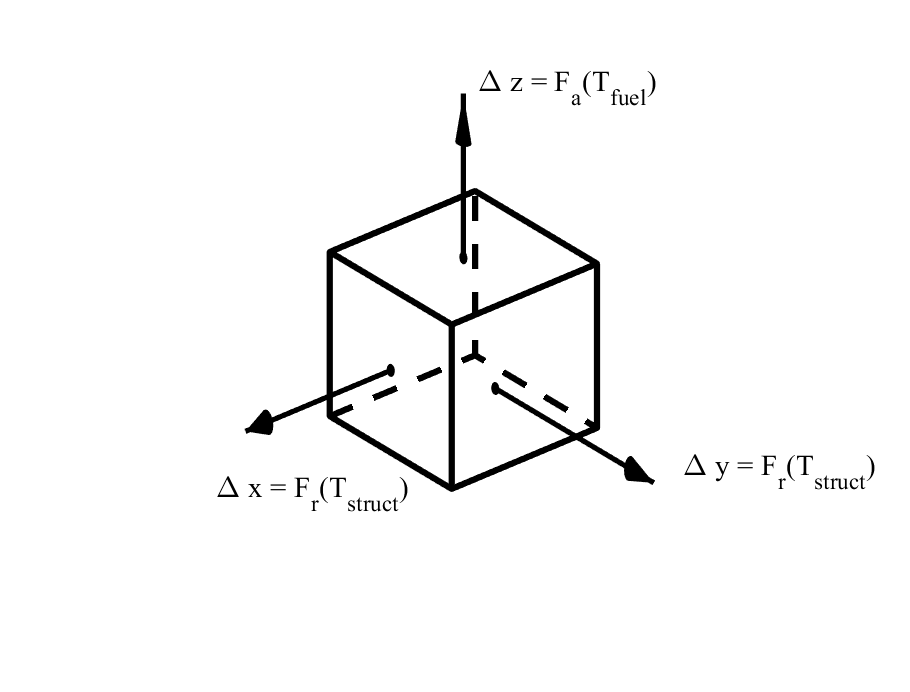
\includegraphics[width=0.7\textwidth]{thexp_figure}
      \caption{Thermal Expansion of General Volume.}
      \label{fig:thexp_figure}
    \end{figure}
    
    For the volume in \fref{fig:thexp_figure}, the thermally expanded 
    volume $V^H$ can be written
    \begin{align}
      V^H &= V^C + \Delta V, \\
      V^H &= (L_x^C + \Delta L_x) (L_y^C + \Delta L_y) (L_z^C + \Delta L_z). 
    \end{align}
    Then, recognizing the coordinate expansions,
    \begin{align}
      V^H &= (L_x^C + L_x^C \, F_r(\texpstruct)) + 
        (L_y^C + L_y^C \, F_r(\texpstruct)) + 
        (L_z^C + L_z^C \, F_a(\texpfuel)), \\
      V^H &= L_x^C \, L_y^C \, L_z^C \, (1 + F_r(\texpstruct))^2
        (1+F_a(\texpfuel)), \\
      V^H &= V^C (1 + F_r(\texpstruct))^2 (1+F_a(\texpfuel)).
    \end{align}
    The volume ratio is then
    \begin{equation}
      \label{eq:volume_ratio}
      \frac{V^C}{V^H} = \frac{1}{(1+F_r(\texpstruct))^2 (1+F_a(\texpfuel))}.
    \end{equation}
    Given the assumption of uniform thermal expansion in axial and radial
    directions, the ratio of volumetric expansion is constant throughout the
    reactor.

    Consider the thermal expansion of fractional areas within a hexagonal
    assembly. The hexagonal assembly has total cross-sectional area $A$ and 
    contains component cross sections with areas $A_i$. For example, the total 
    area occupied by the fuel material could be considered $A_i$ and the total 
    area of the hexagon described by the flat-to-flat dimension could be 
    considered $A$. Define $A_i$ such that $\sum_{i} A_i = A$. Let the 
    fractional area $a_i = A_i/A$ and $\sum_{i} a_i = 1$.

    Using a method similar to the derivation of the volume ratio, a ratio can be
    derived for thermally expanded areas and area fractions. However, this would
    not be useful to the model because within an assembly, not all dimensions
    expand uniformly within the radial direction.
    The fuel radius and fuel area are expanded according to 
    $\left(\frac{\Delta L}{L_0}\right)_{\text{U10Zr}}$ whereas all other 
    materials are expanded according to 
    $\left(\frac{\Delta L}{L_0}\right)_{\text{HT9}}$. This does imply that,
    numerically, the radius of the fuel could exceed the inner radius of the 
    clad which is a non-physical result. This will only happen for small sodium 
    bond gaps and high thermal expansion temperatures. In these cases, the 
    radius of the fuel is confined to the expanded inner radius of the cladding.
    Though a more complex relationship describes the true value of these radii, 
    the error due to this assumption is small compared to the assumption of 
    uniform thermal expansion.
    
    Due to the different thermal expansion rates of fuel and structural material 
    within the cross-sectional area of the hexagonal assembly, the thermal 
    expansion of area fractions does not have a general formulaic relationship.
    Instead, area fractions are simply calculated at hot and cold conditions
    using expanded and unexpanded dimensions respectively. 

\section{Implementation}
  Thermal expansion affects the reactor in two major ways. First, thermal 
  expansion causes the physical dimensions of the reactor to increase. This is 
  modeled by the expansion of individual elements in the solution of the neutron 
  diffusion equation via the FEM
  (see \chref{ch:neutronDiffusion}) as well as the expansion of area fractions
  within the hexagons. Second, as a result in the increase in physical 
  dimensions, the density of reactor materials decreases. This decrease in 
  density is necessary to preserve the quantity of material within the reactor.
  In this derivation, the number of atoms in the reactor are conserved. The 
  density change due to thermal expansion is observed as a decrease in 
  cross-sections.

  \subsection{Expansion of Elements and Area Fractions}
    Given the assumption of constant thermal expansion in radial and axial
    directions, thermal expansion follows immediately. Each node coordinate in
    the unstructured mesh is expanded according to \eref{eq:expand_x}, 
    \eref{eq:expand_y}, and \eref{eq:expand_z}. By expanding in axial and radial
    directions uniformly throughout the reactor, it is certain that there will 
    be no intersection or overlap of elements. As previously discussed in
    \sref{sec:model_details__assumptions_and_formulae}, the thermal expansion of
    area fractions is calculated directly.

  \subsection{Cross-section Effects}
    \label{sec:cross-section_effects}
    The conservation of reactor material is expressed as a conservation of 
    number of atoms. The conservation of the number of atoms for species $i$, 
    can be expressed as
    \begin{equation}
      \label{eq:conservation}
      n_i^H = n_i^C 
    \end{equation}
    where $n_i^H$ is the number of atoms of species $i$ after thermal expansion.
    The number of atoms $n_i$ can be written as 
    \begin{equation}
      \label{eq:nden_definition}
      n_i = N_i \, V_i
    \end{equation}
    where $N_i$ is the number density of species $i$ and $V_i$ is the volume
    occupied by species $i$. Then, inserting \eref{eq:nden_definition} into 
    \eref{eq:conservation} yields an expression for the thermally expanded 
    number density of species $i$ as
    \begin{align}
      N_i^H \, V_i^H &= N_i^C \, V_i^C, \\
      \label{eq:nden_volume_ratio}
      N_i^H &= N_i^C \frac{V_i^C}{V_i^H}
    \end{align}
    where the term $\frac{V_i^C}{V_i^H} < 1$ and represents the expansion of the
    volume occupied by species $i$. 

    The volume $V_i$ can be written in terms of element volume and area
    fraction. Let species $i$ be contained in region $j$ in finite element $e$. 
    This work assumes area fractions are constant within an element and can be
    treated as volume fractions. Then, the volume $V_i$ can be rewritten as 
    $V_i = a_j \, V_e$ where $a_j$ is the area fraction of region $j$ and $V_e$
    is the volume of the element $e$. Inserting this definition for $V_i$ into
    \eref{eq:nden_volume_ratio}.
    \begin{equation}
      \label{eq:nden_expansion_expanded}
      N_i^H = N_i^C \frac{a_j^C}{a_j^H} \frac{V_e^C}{V_e^H}
    \end{equation}
    Recall from \sref{sec:model_details__assumptions_and_formulae} that the
    ratio $\frac{a_j^C}{a_j^C}$ is dictated by the relative expansion of the
    fuel radius and the other structural materials. The area fractions
    themselves are calculated and the ratio is calculated directly. The 
    ratio $\frac{V_e^C}{V_e^H}$ is the standard volume ratio due to thermal 
    expansion and is given by \eref{eq:volume_ratio}. Inserting 
    \eref{eq:volume_ratio} into \eref{eq:nden_expansion_expanded}.
    \begin{equation}
      \label{eq:nden_thexp_update}
      N_i^H = N_i^C \frac{a_j^C}{a_j^H} 
        \frac{1}{(1+F_r(\texpstruct))^2 (1+F_a(\texpfuel))}
    \end{equation}
    Therefore, to preserve the number of atoms in the reactor, number densities
    in the reactor must be updated according to \eref{eq:nden_thexp_update} in
    addition to expanding reactor dimensions. Notice that
    \eref{eq:nden_thexp_update} can also be used to update neutron reaction 
    cross-sections directly as they are proportional to number density according
    to $\Sigma = \sigma N$.

\section{Results}
  The effect of thermal expansion on reactor criticality is observed. As
  previously mentioned in \sref{sec:model_details__assumptions_and_formulae}, 
  the user must input an effective temperature to which the reactor is thermally 
  expanded. This user-input values of $\texpstruct$ and $\texpfuel$ are varied 
  and all other thermal feedback effects are disabled in the simulation. It is 
  expected that thermal expansion will cause a significant decrease in $\keff$ 
  and represent negative reactivity insertion. Effective neutron multiplication 
  factor as a function of thermal expansion is plotted in \fref{fig:thexp_study} 
  and the associated reactivity, calculated as
  \begin{equation}
    \label{eq:reactivity_formula}
    \rho \units{pcm} = \frac{\keff - \kref}{\keff \, \kref} \times 10^5
  \end{equation}
  is plotted in \fref{fig:thexp_study_reactivity}. In
  \eref{eq:reactivity_formula}, $\keff$ is the calculated effective neutron 
  multiplication factor after thermal expansion and $\kref$ is the neutron 
  multiplication factor without thermal expansion. 

  Given the assumptions in this model, \fref{fig:thexp_study}  and
  \fref{fig:thexp_study_reactivity} show that thermal 
  expansion represents a significant reactivity effect and contributes as much 
  as $-1,000 \units{pcm}$ at extreme temperatures. Additionally, in this model 
  the thermal expansion factor of the fuel given in \eref{eq:lef_u10zr} 
  dominates and the phase change given by the formula can be seen at the 
  expected $923 \units{K}$.

  \begin{figure}
    \centering
    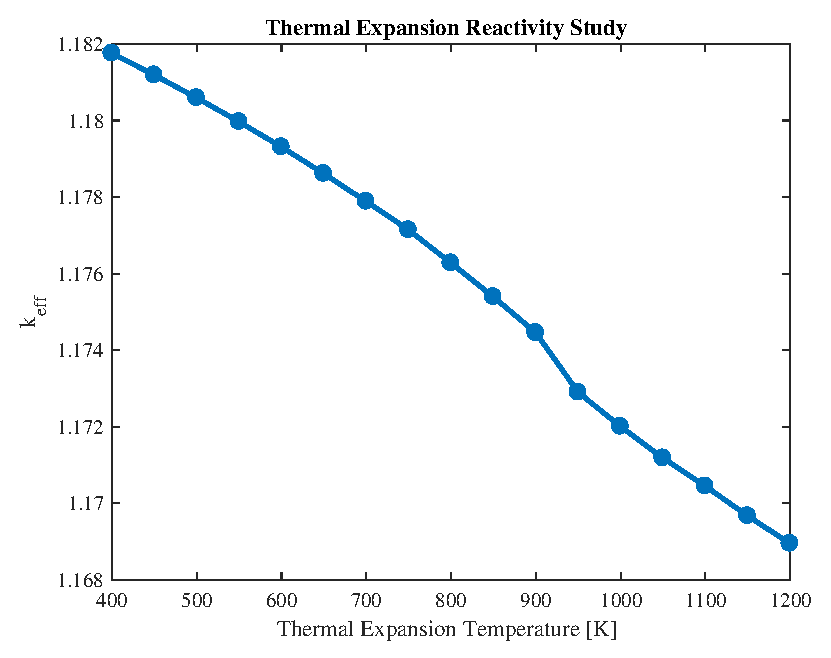
\includegraphics[width=0.7\textwidth]{thexp_study}
    \caption{Effective Neutron Multiplication Factor as a Function of 
      Thermal Expansion Temperature.}
    \label{fig:thexp_study}
  \end{figure}

  \begin{figure}
    \centering
    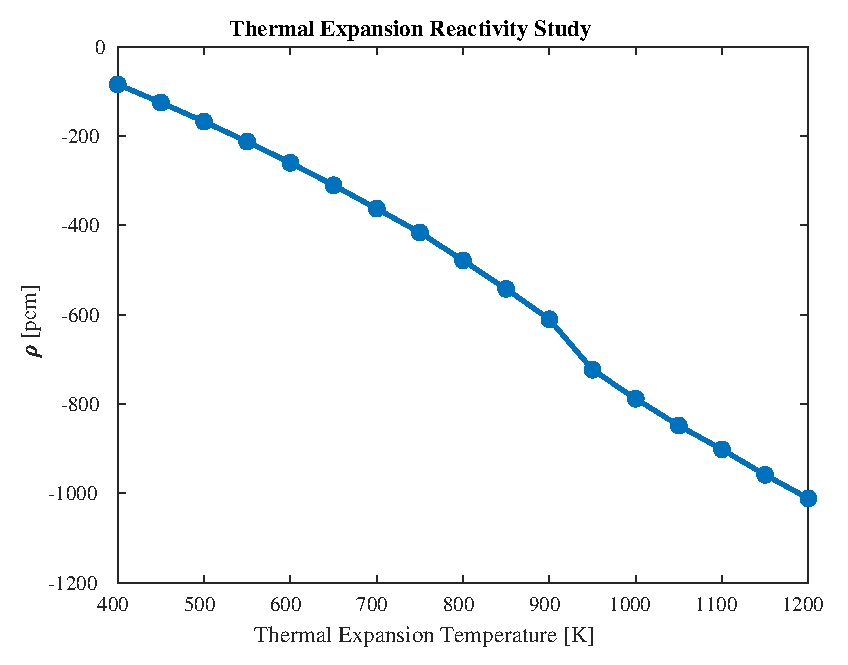
\includegraphics[width=0.7\textwidth]{thexp_study_reactivity}
    \caption{Reactivity as a Function of Thermal Expansion Temperature.}
    \label{fig:thexp_study_reactivity}
  \end{figure}
